\section{Background and related work}
We cover the background of far memory solutions and why they are important followed by the current state of prefetching and CHERI.

\subsection{Far memory}

% Current state of far memory systems and why they are necessary.
Far memory devices are devices used to store application memory pages that are not directly addressable from the processor using regular instructions i.e., load and store. Currently, most systems~\cite{google,meta,fastswap,infiniswap} use z-swap~\cite{zswap-1}, SSDs, or disaggregated memory~\cite{leap, infiniswap} (DRAM over a network) as their far memory solutions. Z-swap compresses a page of memory and stores it in a compressed form in DRAM, whereas in the case of SSDs and networks, the entire page is written on the SSD or over the network, typically using RDMA. There are many ways to expose the backends to applications. One transparent method uses the swap subsystem inside an Operating System. When the application's working set cannot fit in the allocated memory, the operating system swaps out inactive pages to the swap backends. Datacenter operators use mechanisms (such as \texttt{cgroups} in Linux~\cite{cgroups}) to restrict the memory usage of individual applications running on a system. When the memory allocated to an application is exhausted, the Operating system transparently swaps out memory pages to swap to make space for new pages.  

% Far memory systems implementation in datacenters.
The key challenge datacenter operators face is that they need to control the performance impact of using Far Memory to meet SLAs. This poses a significant challenge. A good far memory implementation makes these key decisions --- 
\begin{enumerate}
    \item What percentage of pages of an application to offload
    \item Which pages to offload 
    \item Which swap backend or memory technology should be used
    \item Which pages to prefetch based on application behavior
\end{enumerate} 

% Different approaches of page eviction used in these systems.
% The performance impact can be controlled in one of the following ways --- (1) By controlling the percentage of pages that are swapped out to far memory for each application. (2) Selecting which particular pages to swap out, cold pages have less impact on performance than hot pages. (3) Using a prefetcher that has good coverage and accuracy. The first two parts are controlled by the eviction algorithm which we will cover in detail in the following section.

% What optimizations exist on the swap path for far memory
Swap systems work transparently to the application. There are three major components of importance in this path, eviction, and prefetching. We focus on the prefetching. 


% Systems have attempted to optimize the number of pages to be swapped out. In an environment where it is unclear how many pages can be swapped out without having a performance impact on the application, dynamic decisions need to be made. G-swap fixed a percentage of application pages based on offline analysis and TMO uses a dynamic metric called Pressure Stall Information (psi) to decide the percentage of pages which can be swapped out without an impact on application performance. Many approaches exist to decide which pages are cold, G-swap walks the page table every 120 seconds and checks which page has been accessed in that duration and marks them as hot. TMO uses the default linux mechanism which is based on the LRU-2Q algorithm and does partial page tracking based on active and inactive queues. The current linux algorithm is efficient and uses less than 0.01\% of CPU cycles. 

\subsection{Page prefetching}
% Current state of linux prefetchers
Page prefetchers are deployed in most modern Operating systems to reduce the latency of page access from swap. Typically the important prefetching metrics are accuracy, coverage and timeliness. Accuracy is the ratio of prefetched pages to prefetched pages accessed. Coverage is the ratio of pages prefetched to the pages accessed by the application. Timeliness refers to the difference between when a page was prefetched and when it was actually accessed by the application. Prefetched pages are put in a datastructure (cache) often called the Pagecache. Linux implements a prefetching algorithmn based on virtual address that focuses on spatial locality of virtual addresses~\cite{vma-readahead}. Though this algorithm works for many applications, it doesn't work for workloads that don't show these characteristics, Leap~\cite{leap} improved upon Linux in many aspects. We talk about Linux in this section but all the techniques and algorithms are the same in FreeBSD and CheriBSD~\cite{cheribsd}.

% Leaps improvement on linux
Leap introduced an approximation based algorithm based on the Boyer-Moore majority voting algorithm applied to the page access history of an application. They also implemented a mechanism to invalidate pages in the PageCache when they are accessed, to reduce cache pollution and free up space for more pages (PageCache size is usually 32Mb). Using a combination of these techniques, Leap improved upon Linux by upto 10\% in prefetcher accuracy and coverage and 30\% reduction in application execution time. Leap improved upon Linux for many applications but still focuses on spatial locality and ignores accesses that don't follow a pattern.

% Canvas and memliner and the issues of leap they fixed. 
Canvas~\cite{canvas} and Memliner~\cite{memliner} improve upon Leap by addressing the issue of separating access patterns of different threads. Canvas introduces a new mechanism to isolate the swap subsystem and the memory access histories of threads inside the kernel. Additionally, it introduced a mechanism in the OS to issue an upcall to the application (JVM for Canvas) if the OS cannot decide pages to prefetch, The application can use additional insight to decide pages to prefetch, for example they made a prefetcher for Java by locating the object corresponding to the faulting address and prefetching the data inside that object. Memliner improved prefetcher accuracy and coverage for managed languages where GC memory accesses interfere with application accesses. Since the OS cannot dinstinguish between the GC accesses and application accesses, these interleaving histories make it difficult to find a pattern. Memliner, aligns the memory accesses from both the GC and the application, i.e. GC memory accesses are ordered in a way that they don't interfere with the application access history. This technique increases the efficiency of Leap.

\subsection{CHERI}
CHERI is an architecture extension that complements the page access based protection model used in most Operating Systems. CHERI maintains the Load/Store model of RISC and implements hardware based memory protection. Each pointer that is created as a capability in CHERI is 128 bits. The first 64 bits of a pointer are treated as a regular pointer, but the other 64 bits contain information needed by hardware to enforce protection for memory accesses. For example, when a memory address is accessed, CHERI will load the 64bit value to a capability register, using this value the hardware can check for various security features such as bounds checking, pointer integrity, etc. Additionally, for each capability, the architecture also stores a tag bit in memory, which indicates that the location in memory contains a capability. In "purecap" mode, every pointer of an application is treated as a capability, giving the hardware fine-grained information about what memory ranges the application can access. The CHERI instruction set also provides an instruction to read the tag bit which provides the ability to identify pointers stored in memory. This instruction was used by Cornucopia~\cite{cornucopia} and CHERIvoke~\cite{cherivoke} to prevent temporal memory bugs (such as use after free) in an efficient way at runtime. In contrast, we use the instruction set to increase prefetching performance for an application. 
\textbf{CheriBSD and swap modifications -} Currently, there is a port of FreeBSD that fully supports CHERI capabilities. For an Operating System to be CHERI capable i.e., can be compiled to CHERI, certain coding standards need to be followed and changes to some subsystems are necessary. CheriBSD is fully compatible with CHERI and to support that modifications need to be made to the Operating System, we focus only on swap subsystem modifications. When a memory page is swapped out, it might contain capabilities (pointers) inside the page, since those are not accessible anymore, the hardware tag bit needs to be cleared for those pointers. Currently, CheriBSD will store these tag bits as a bitmap inside a trie. When a page is swapped back in, the hardware tag bit needs to be reset. The OS will read the bitmap in the trie and restore the tag bits for all the capabilities present inside this page. This added overhead is because of using CHERI as an architecture and cannot be avoided.

\begin{figure*}
\caption{CHERI-picking is effective in prefetching patterns that the kernel prefetcher cannot. Second bar shows that allocation order requires the kernel prefetcher to be preferred.}
\label{fig:evaluation}
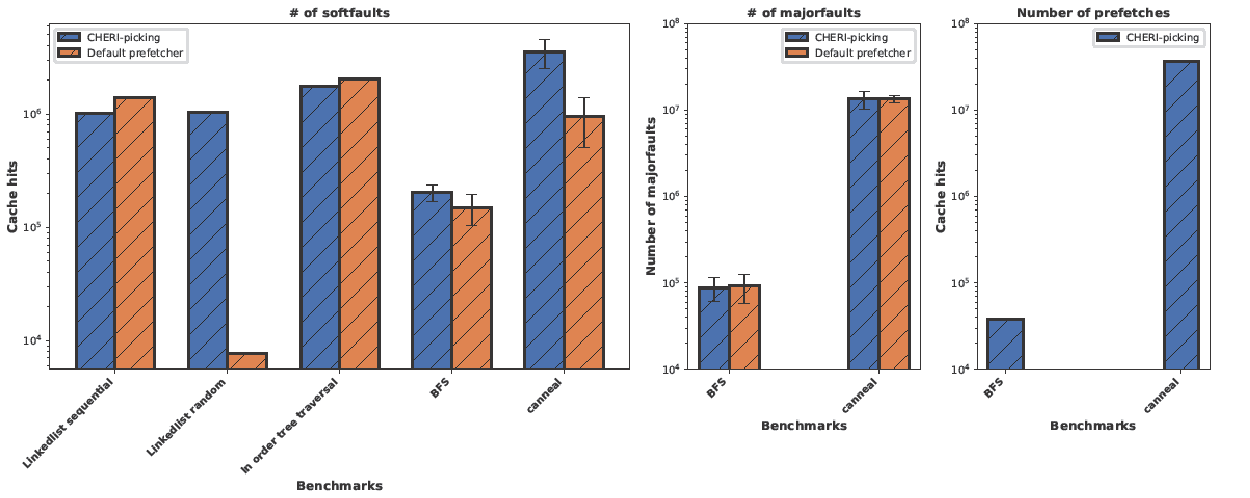
\includegraphics[width=18cm]{images/evaluation_graphs_cropped.pdf}
\centering
\end{figure*}